
\documentclass[
12pt, % The default document font size, options: 10pt, 11pt, 12pt
%oneside, % Two side (alternating margins) for binding by default, uncomment to switch to one side
english, % ngerman for German
singlespacing, % Single line spacing, alternatives: onehalfspacing or doublespacing
%draft, % Uncomment to enable draft mode (no pictures, no links, overfull hboxes indicated)
%nolistspacing, % If the document is onehalfspacing or doublespacing, uncomment this to set spacing in lists to single
%liststotoc, % Uncomment to add the list of figures/tables/etc to the table of contents
%toctotoc, % Uncomment to add the main table of contents to the table of contents
parskip, % Uncomment to add space between paragraphs
%nohyperref, % Uncomment to not load the hyperref package
%headsepline, % Uncomment to get a line under the header
]{MastersDoctoralThesis} % The class file specifying the document structure

\usepackage{float}
\usepackage[utf8]{inputenc} % Required for inputting international characters
\usepackage[T1]{fontenc} % Output font encoding for international characters
\usepackage{titlesec}
\usepackage{palatino} % Use the Palatino font by default
\usepackage[backend=bibtex,style=authoryear,natbib=true]{biblatex} % User the bibtex backend with the authoryear citation style (which resembles APA)

\addbibresource{example.bib} % The filename of the bibliography

\usepackage{graphicx}
\graphicspath{ {Chapters/images/} }

\usepackage[autostyle=true]{csquotes} % Required to generate language-dependent quotes in the bibliography

%----------------------------------------------------------------------------------------
%	MARGIN SETTINGS
%----------------------------------------------------------------------------------------

\geometry{
	paper=a4paper, % Change to letterpaper for US letter
	inner=2.5cm, % Inner margin
	outer=3.8cm, % Outer margin
	bindingoffset=2cm, % Binding offset
	top=2.5cm, % Top margin
	bottom=2.5cm, % Bottom margin
	%showframe,% show how the type block is set on the page
}

%----------------------------------------------------------------------------------------
%	THESIS INFORMATION
%----------------------------------------------------------------------------------------

\thesistitle{TODO: insert a title here} % Your thesis title, this is used in the title and abstract, print it elsewhere with \ttitle

\supervisor{Dr. Germano \textsc{Bonomi}} % Your supervisor's name, this is used in the title page, print it elsewhere with \supname
\examiner{} % Your examiner's name, this is not currently used anywhere in the template, print it elsewhere with \examname
\degree{Master degree in Computer Engineering} % Your degree name, this is used in the title page and abstract, print it elsewhere with \degreename
\author{Andrea G.B. \textsc{Damioli}} % Your name, this is used in the title page and abstract, print it elsewhere with \authorname
\addresses{} % Your address, this is not currently used anywhere in the template, print it elsewhere with \addressname

\subject{  } % Your subject area, this is not currently used anywhere in the template, print it elsewhere with \subjectname
\keywords{} % Keywords for your thesis, this is not currently used anywhere in the template, print it elsewhere with \keywordnames
\university{\href{http://www.unibs.it}{}} % Your university's name and URL, this is used in the title page and abstract, print it elsewhere with \univname
\department{\href{}{}} % Your department's name and URL, this is used in the title page and abstract, print it elsewhere with \deptname
\group{\href{ }{ }} % Your research group's name and URL, this is used in the title page, print it elsewhere with \groupname
\faculty{\href{ }{ }} % Your faculty's name and URL, this is used in the title page and abstract, print it elsewhere with \facname

\hypersetup{pdftitle=\ttitle} % Set the PDF's title to your title
\hypersetup{pdfauthor=\authorname} % Set the PDF's author to your name
\hypersetup{pdfkeywords=\keywordnames} % Set the PDF's keywords to your keywords

\titlespacing*{\subsection}
{0pt}{10.5ex plus 1ex minus .2ex}{4.3ex plus .2ex}

\begin{document}


\frontmatter % Use roman page numbering style (i, ii, iii, iv...) for the pre-content pages

\pagestyle{plain} % Default to the plain heading style until the thesis style is called for the body content

%----------------------------------------------------------------------------------------
%	TITLE PAGE
%----------------------------------------------------------------------------------------

\begin{titlepage}
\begin{center}

\textsc{\LARGE \univname}\\[1.2cm] % University name

{\huge \bfseries \ttitle}\\[0.4cm] % Thesis title
\HRule \\[1.5cm] % Horizontal line
 
\begin{minipage}{0.4\textwidth}
\begin{flushleft} \large
\emph{Author: 
}\\
\href{}{\authorname} % Author name - remove the \href bracket to remove the link
\end{flushleft}
\end{minipage}

\begin{minipage}{0.9\textwidth}
\end{minipage}

\begin{minipage}{0.4\textwidth}
\begin{flushleft} \large
\emph{Supervisor:} \\
\href{}{\supname} % Supervisor name - remove the \href bracket to remove the link  
\end{flushleft}

\end{minipage}

\begin{minipage}{1.9\textwidth}
\end{minipage}
 
%{\large \today}\\[4cm] % Date

\centering 
\hfill 
\begin{minipage}[b]{.3\columnwidth} 
  \centering 
  {\large Master Thesis}\\[4cm]  
\end{minipage}\hfill 
\begin{minipage}[b]{.3\columnwidth} 
  \centering
  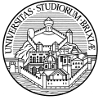
\includegraphics{Logo} 
\end{minipage}\hspace*{\fill} 

 % University/department logo - uncomment to place it

\vfill
\end{center}
\end{titlepage}

%----------------------------------------------------------------------------------------
%	ABSTRACT PAGE
%----------------------------------------------------------------------------------------

\begin{abstract}
\addchaptertocentry{\abstractname} % Add the abstract to the table of contents

%The Thesis Abstract is written here (and usually kept to just this page). The %page is kept centered vertically so can expand into the blank space above the %title too\ldots

The AEgIS Experiment at the CERN aims to verify the weak interaction principle for antimatter. This document talks about "gAnWeb", a web application designed to simplify the analysis of physical data under the AEgIS experiment. This analysis can be performed using Root Data Analysis Framework by the Linux Terminal using an application named "gAn", but a graphical interface can ensure a better user experience, ease the user training and improve the productivity. This document analyses from the Human Machine Interaction's point of view the production of this graphical interface.  

 
\end{abstract}


%----------------------------------------------------------------------------------------
%	LIST OF CONTENTS/FIGURES/TABLES PAGES
%----------------------------------------------------------------------------------------

\tableofcontents % Prints the main table of contents

%\listoffigures % Prints the list of figures

%\listoftables % Prints the list of tables


%----------------------------------------------------------------------------------------
%	THESIS CONTENT - CHAPTERS
%----------------------------------------------------------------------------------------

\mainmatter % Begin numeric (1,2,3...) page numbering

\pagestyle{thesis} % Return the page headers back to the "thesis" style

% Include the chapters of the thesis as separate files from the Chapters folder
% Uncomment the lines as you write the chapters

% Chapter 1

\chapter{Introduction} % Main chapter title

\label{Chapter1} % For referencing the chapter elsewhere, use \ref{Chapter1} 

%----------------------------------------------------------------------------------------

\section{User friendly Data analysis: gAn Web}

GAn is a program that aims to analyse data related to the AEgIS experiment at the CERN, gAn Web is the web interface of gAn, and it is the main topic of this document.
 
This program receive in input (from another software system) several terabytes of files in ".root" format, and some input parameters inserted by the user; 
It does an analysis and it gives in output some summarized scientifically interesting information, understandable by humans.   
A file ".root" is a file produced by a variegated group of sensors in a complex machine that accelerates particles and lets them crash together. This sensors produce data continuously (8 hours per day), and a software system validates and saves these data in file with .root extension. 

The input parameters are:
\begin{enumerate}

% 1
\item "Run Number", that identifies in which part of the data the user is interested. 
The time in this experiment is divided in "runs" (a run lasts about some hundred seconds), so the user, by the run parameter can tell to gAn in which time slice he is interested. For example: run 55614 means that the user is interested in the information related to the 22th of November 2016, taken in the time slice between 15:45 and 15:47. The enumeration of the runs is incremental: so the run 55199 identifies the time slice immediately after the time slices identified by 55198. This system to identify time slices seems to be strange at the beginning but is a standard for all the applications in the AEgIS experiment and it allows a very efficient and precise communication.
 

% 2
\item "Type of analysis", that identifies what the program must do with the data and what it must show as output to the user.
A "type" is a way in which the program extracts information from the raw data. each type can extract different information using different parts of data and elaborating them in different ways. For example: a type of analysis named "Tmeas" can extract information about the temperatures of some elemental particles analysing how quickly they move subjected to a force. 

\end{enumerate}


The .root files can be analysed using a framework named ROOT Framework, that consists in a lot of libraries specialized in high-energy physics analysis, and an interpreter able to understand a C++ script.
Actually, gAn is the sum of the Root Framework plus a lot of C++ scripts.
The goal of gAn is reduce the big amount of raw data received in input in a little amount of scientifically interesting and easily understandable data in output. To do this it has to filter data, understand which of them are scientifically interesting, chose the parts that are related to the run selected by the user (by the run parameter), elaborate and compare them, and make advanced statistical analysis on them.  
gAn can be called using a common linux terminal, using a command with parameters. 

The output of gAn consists of a single text file with computed, (quite) organized data, and a folder of images in png format.
This structure (root files in input, data analysis using Root, images, organized and selected data in output) is very common in the CERN's experiments. 
The output of gAn is quite understandable by an experienced physicist, but it is disorganized, complex for an untrained user, and the terminal interface can be surely improved using some more user friendly technologies.

GAn Web is a web application, that aims to create a user friendly web interface, based on the most important human-machine interaction principles, between the users and gAn.
A web interface can improve the system in two ways:

\begin{enumerate}

% 1
\item gAn is a stand-alone program based on Root, installable on the user's machine; the user has to install the correct version of Root to avoid compatibility problems (Root is still not perfectly version independent: different versions can lead to different behaviours). Furthermore, this kind of program is continuously changing, the performed analysis is continuously improved (in the first 2 weeks from the debut of the program there are already several different kinds of analysis, because often at the changing of the needs the programmers creates new generations of analysis), so the installed version of gAn is not final and unchangeable, and the user musts often update it. Instead, a centralized version installed on a server, with services accessible from a normal browser by the user can avoid (at least reduce) this kind of problems and be more usable.    
 

% 2
\item a Linux terminal interface is practical for expert users, but a web based interface can be more attractive for new users, and, if well done, can be easier to use. It is important to notice that the users are physicists, not necessarily specialized in computer science, so, create a friendly and easily learnable interface can avoid them problems and time wasting.   


\end{enumerate}


The goal of gAn Web is to allow users to do analysis through a more friendly web interface, without install nothing on their machine. In the following image there is a schema that shows how this program is organized.

\begin{figure}[H]
\centering
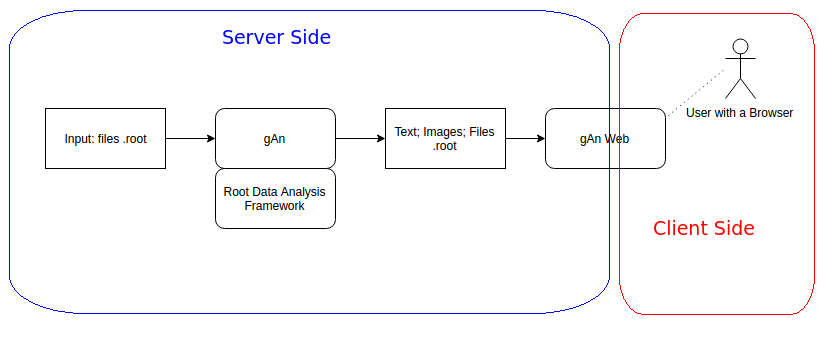
\includegraphics[scale=0.5]{GeneralGAnSchema.png} 
\caption{gAn - gAn Web simple scheme}
\end{figure}




% Chapter 1

\chapter{Requirements} % Main chapter title

\label{Chapter2} % For referencing the chapter elsewhere, use \ref{Chapter1} 

%----------------------------------------------------------------------------------------

First of all is important to analyse which are the requirements of gAn web (and how gAn web can improve the performances of gAn). 

\section{The role of the designer and the users}
In this design process the interaction between designer and users is very strict: in fact for about 2 months, divided in blocks of more of less 2 weeks, the designer has worked together directly with the users. 

It is interesting to note that the domain in which this application works is quite complex and different from the domains in which the designer is specialized, so, some periods of work directly with the users are necessary to let the developer understand better how does the domain works.
This period of time allowed the designer to understand better how exactly the work processes take place, and what are the needs of the users. 
It is important to precise that this kind of users is quite particular: their education level is very high (almost all of them have a Phd), and their need are very specialized (related with the physics research world).

In this design process we can identify 3 main actors: 
\begin{enumerate}

\item
The designer, who produced the web interface (gAn Web)

\item 
Two pilot users (university professors in Brescia), that are also co-developer of the application behind this interface (gAn). So they act both the role of the users, and the role of the supervisors. 

\item A group of users (around 10-12) in Geneva. This main group is used for the final testing of the application.
 
\end{enumerate}

The design process can be also divider in three stages:

\begin{enumerate}

% 1
\item An early stage, more simple, with basic functionalities, just to investigate what are the best ways to implement the functionalities and to test with the little group of pilot-users (two) if this software can really be useful and which functionalities are really important; The goal of this stage is to give an initial direction to the development and improve the designer's knowledge of the domain. At the end of this stage, the test with the two pilot users helps to correct the way.

% 2
\item An intermediate stage, more complex, with some advanced functionalities obtained listening the request of the pilot users. This version is installed in the AEgIS control room and the users use it. 
The designer needs at this point to execute some test with the maximum possible number of users to understand if the product is acceptable and useful (and how to improve it). 
The tests with the users show a lot of useful information and allow the developer to find a big group of problems: the solutions to these problems give the birth at the final version. 

% 3
\item
The third stage is the final stage. At this point the application is modified to accord the observations of the users. It is important to notice that the third stage (the last one) is a never-finished stage: the needs of the users are permanently changing and evolving, the application is designed to be adaptable, and to try to satisfy the unknown needs of future users.

\end{enumerate}

\section{Functional requirements}
The definition of functional requirements aims to specifying in detail what the web application can do, and in which way an user can use it. The development of gAn web is divided in three stages, so the requirements are peculiar and different for each stage, and following they are exposed divided in the three groups: 

\subsection{Early version}
The first version (from now "gAn web v1") is a very simple application: instead of access the program by a linux terminal like gAn, in gAn web v1, the user can 
use the program through a graphical interface. 
The requirements of this version are the following:
\begin{enumerate}

% 1
\item The user, in the homepage, can chose the run (only one run, for the moment) in which he is interested, using a input field. This field has validator, able to understand if the run number is inserted, if it is effectively a number, and if it is in an acceptable range. The user receives an explaining and precise error message directly on the homepage if the input field is empty and if the inserted value is not acceptable. It is always possible validate the inserted run and ensure that the related Root file exists? No, because in some moments some sensors don't work properly and it is inevitable that some root files related to some runs are incomplete, or even inexistent.

% 2
\item At this moment there is only a generic idea about what kind of analysis can be useful for the user, so in this version there will be only a generic analysis, able to dump in text all the possible information, and a group of example images (this is useless for the goal of the scientific research, but very useful to improve the understand the needed features of the web interface).
At this stage is not clear if the type of analysis will be chosen by the user of automatically selected by the program , so in gAn web v1 there are no buttons able to allow the user to select the type of analysis (this point will be reconsidered in next versions).

% 3
\item The user can start the program with a single click, by a button (usable only if the inserted number is valid).

% 4
\item When the program is executed the user can see the text output on the screen. This text is clear for a physicist (it is not clear for a person who doesn't have a specific preparation). 

% 5
\item When the program is executed the user can see the output images by clicking a button that link to a images-page. The images are ordered and organized by groups (the groups are related about which sensor takes the information necessary to create the image). The user can decide if he prefers to see the image in a little, medium or big format. The user can also decide if the images are distributed in the screen vertically or through a "carousel layout". The user can access the image in full-screen by clicking on it: he is redirected to a page with the image shown in full screen, and can return back to the all-images page by a return button. It is absolutely important to understand exactly which information are interesting for the users, and show in the images only them and all of them, this point will be solved with a confrontation with the pilot-users. 

%6
\item The user can modify a configuration file (a .txt file on the server), by a web interface. In this files there are some values the need to be setted (otherwise it uses default values), and the user can do it by radio buttons (in this way he is forced to chose valid values). This configuration file can modify the way in which gAn works and modify the resulting output (both the text and the images).   

\end{enumerate}

\subsection{Intermediate version}
The intermediate version (from now "gAn Web v2") is more complex. It was born from the tips and the observation of the pilot users. The modifications are not numerous, but there are a lot of additions of new features. All the new required characteristics are exposed following:

\begin{enumerate}

% 1
\item The user can insert multiple runs: separated by a semicolon (but in case of errors the system can automatically correct them replacing symbols like "-" or "," or "." with semicolons and giving a more robust service). These runs can be inserted by an input field of by a range select button: this button open a "modal" that allows the user to chose the first run and the last, and automatically insert the comprised runs (for example, if the user inserts 30000 and 30010 the system inserts automatically all the run numbers between 30000 and 30010). This modal has a validation system, that ensure the correctness of the inserted values. It is not perfectly clear if this solution fit the needs of the users, but the tests with the whole users group will probably solve this doubt. 

% 2
\item The user can chose which kind of analysis execute. At this point the different analysis are related to the different branches of gAn that at this stage an heterogeneous group of programmers are developing and uploading on Gitlab. It is no clear which of these branches will be definitive and which no, lo the program must be able to use all of them. The type of the analysis depends on the version of gAn downloaded and used for the execution of the program. In gAn Web v2 five complete branches exist, but in the future they can became more. They are externally very similar, the differences are the algorithms in the program, but they give a different output (different output but in the same format: text and images). 
At this stage is not clear if all this different versions will be used for the final application, to clarify this point the best solution is observe directly the user's behavior. 

% 3
\item The configuration file is not only in text format, but also can be in xml format (it depends on the selected version of gAn). The xml ensures a stronger structure, and must be transparent to the user (he mustn't see differences between the configurator that works with a txt file and the one that works with xml). At this stage both text format and xml format are acceptable, to ensure the retro-compatibility of some analysis, but is possible that in further versions the xml-based design will became dominant. 

%4
\item The user can chose what version of Root he wants to use for the program. Theoretically different versions of Root are perfectly compatible, but in practice each version of gAn is designed to work with a particular version of Root and to avoid problems it seems to be a good idea to allows the user to choose freely which version of Root use among the installed versions on the server.  

%5
\item The user can save images on his hard disk: he can chose from the shown images in the images page an image to download by clicking on a specific download button near the image. Furthermore there is another button "Download All" with whom the user can simple download all the output images.

%6 
\item The user can download a reduced version of the root file with informations about the images and the results: gAn produce this kind of files as "half-processed" during the computing, and it is not a problem to save this on the hard disk of the server in a specified folder. For an expert user can be scientifically interesting have this file (this root file contain more information than the output, the most of this information is useless [it is an "half-processed" file] , but sometimes an expert user can find something interesting), so the user must have the opportunity to download this.     

% 7
\item The first little group of user prefers the dropdown menu to the radio button, so all the radio buttons in the program are replaced by dropdown menus.

% 8
\item The user has to access not only to a png image, but to a root-image. This kind of image is interactive: the user can with a left click of the mouse (a continued click, like the "dragging") select parts of the image and zoom them, and with a right click do dynamically some kind of image processing (set colors, chose  what kind of chart to show, modify the chart legend, translate in a 3D space the image etcetera). In this way each user can choose freely which information he wants see in the image (try to overseen user's needs in this part seems to be too difficult and not useful).
All of this must be done by the user through a browser window. This requisite seems to be quite complex, but Root provides libraries (these libraries work well but they are poorly documented) to interact with Javascript, and can in some way resolve the problem.  

% 9
\item In the homepage the user can see the run number of the last root file produced by the machine, and its creation date and time (so, he can understand what is the maximum of the range of the insertable numbers). Also, the run number is an unit of measurement of the time, so through this number the user can have information about the progress of the experiment.  

In the intermediate version there was another functional requisite: ideally the user should have been able to select a gAn version also if not installed in the server machine: in this case the system should have been capable to automatically search on the AEgIS Gitlab repository the correct version (if existing), download it, unpack it in the server, and use it to execute the program. 
After some discussion this requirement has been cancelled, because it was considered complex, basically useless, and potentially harmful (on the branches of the repository there are untested and incomplete versions, that can create if executed wrong outputs, so wrong scientific results). At this moment installing manually the stable versions of gAn on the server seems to be a more smart way to work.

% 10
\item There is a login system: the user must insert the password of the office to use the system. The authentication is based on the confrontation between the hash function of the inserted password and the hash function of the AEgIS password. If the password is correct the user receives a cookie, before each action in the site the server request and check this cookie to be sure about the identity of the user.  


\subsubsection{Ambiguities (and related solutions)}

At least a point seems to be quite ambiguous: 

The textual output of gAn needs to be formatted in some way to be more organized and clear? 
The answer is difficult: for a non-physicists this output seems to be disordered, too long, with too many groups of informations, and very difficult to understand, but on this question the pilot users (that are physicists) questioned answered that the output is perfectly clear and doesn't need to be modified or improved in any way. The only requests of the users were about the font and the font-size. To check this fact the best solution probably is observe the behavior of the users at work, and eventually ask them informations about that.
Anyway, in the second version, in case of multiple run selection, there is a "navbar" that allows the user to show only a run-result per time.


\end{enumerate}

\subsection{Final version}
The last version (from now "gAn Web v3") is a modified version of the intermediate version. 
The second version's modification come from two sources: some adding requirements are proposed from the pilot users (that are also supervisors); These adding requirements are the following:

\begin{enumerate}
%1 chose analysis new way
\item 
The main kinds of analysis are now more clear: they are 4-5, and they are     quite stable. Their role and when they are useful is now steadily fixed. Each user, according on his task, knows (should know) in every moment which analysis fits better the situation, so, the best solution is allows the user to choose the type of the analysis through a dropdown menu directly in the main page (exactly like he chooses the run number). At this point the possibility of choose the gAn version is useless, because the definitive version of gAn include all the existing types of analysis. 

%2 single vs multiple
\item 
The kind of use of this software is quite different if you decide to work with a single run or a group of runs, so is better if at the beginning the user chose directly if he wants work with a single run or more than one. 

%3 don't choose root version
\item
There is an effort in the developing of the whole project to make it independent of the Root version, So the interface won't ask to the user to choose a Root version anymore.

\end{enumerate}
 
Furthermore, the version version with this last requirements was tested with the users: the developer studied their behavior observing them at work with the existing version, listening to their comments, and asking them opinion and information. The impact  of the debut with the users highlights some problems to be overcome, and from the analysis and the solution of these problems the requirement of the last version was defined. The problems observed (and for each the proposed solution) are the following:

\begin{enumerate}
\item 
It is important to help the user in some way to choose the run number: the user needs a view on the logbook of the run, that is a text in which there are information about each run number divided by date.

\item
Actually nobody use the button to modify the dimension of the images: they all use the biggest version.. is better to remove (or move in a less central place) this dropdown. A similar reasoning can be done for the dropdown that allows the user to switch between the vertical and carousel menu (everybody use).

\item
The read of the textual output takes too much time: it can be improved highlighting the most important parts (or better, the most important parts for the selected type of analysis)

\item
The user need to choose by the configuration page the degree of precision (the minimal error) of the x-axis (the time related axis) of each time-related values images. This parameter seemed to be not very important and in the second version actually there wasn't, but all the users modifies it quite often (manually). So is better to let them to do it by the interface

\end{enumerate}
 
\section{Non-functional requirements}

Both versions, the first and the second, have some non-functional requisites:

\begin{enumerate}

\item The first is quite simple: gAn web has to ensure that in case of crash of the program the web server mustn't crash too. The point is that on this web server (Apache server, installed on Linux) there are some other important applications, so, if gAn web crashes it is not a big problem, but the crash cannot force Apache, or worst the entire machine, to stop or restart. 
This requisite is quite easy to meet: a modern web application based on Html, Javascript, PHP and CSS is quite safe, a general crash of the server it is very unlikely to happen. If the C++ application or some Root libraries crashes (for example if the user asks for an inexistent run) the web application gracefully warn the user about the problem, but without uncontrolled behaviours.  

\item The application must work without install nothing. Also this requirement is very easy to meet: gAn Web is a web interface, it requires only a browser, nothing else.

\item The application must be compatible with any machine (except mobile phones, not requested), regardless of hardware, operating system, installed software. Also this requirement is achieved because of gAn Web only needs a browser to be used. 

\item The application must be easy to be modified and extended in the future by persons who aren't necessarily software engineers. The point is that the student who wrote this program is a "momentary collaborator" in the AEgIS experiment, and all the modifications to the program must be done by other people, in most cases physicists. So the best way is to comment in detail the code and keep the code simple (this is a basic good-programming requirement).   


\end{enumerate}


% Chapter 1

\chapter{Early version} % Main chapter title

\label{Chapter3} % For referencing the chapter elsewhere, use \ref{Chapter1} 


At this point is important to analyse which are the requirements of gAn web at the first version:

\section{Functional requirements}
The definition of functional requirements aims to specifying in detail what the web application can do, and in which way an user can use it. The development of gAn web is divided in three stages, so the requirements are peculiar and different for each stage. The first version (from now "gAn web v1") is a very simple application: instead of access the program by a linux terminal like gAn, in gAn web v1, the user can use the program through a graphical interface. 
The requirements of this version are the following:

\begin{enumerate}

% 1
\item The user, in the homepage, can chose the run (only one run, for the moment) in which he is interested, using a input field. This field has validator, able to understand if the run number is inserted, if it is effectively a number, and if it is in an acceptable range. The user receives an explaining and precise error message directly on the homepage if the input field is empty and if the inserted value is not acceptable. It is always possible validate the inserted run and ensure that the related Root file exists? No, because in some moments some sensors don't work properly and it is inevitable that some root files related to some runs are incomplete, or even inexistent.

% 2
\item At this moment there is only a generic idea about what kind of analysis can be useful for the user, so in this version there will be only a generic analysis, able to dump in text all the possible information, and a group of example images (this is useless for the goal of the scientific research, but very useful to improve the understand the needed features of the web interface).
At this stage is not clear if the type of analysis will be chosen by the user of automatically selected by the program , so in gAn web v1 there are no buttons able to allow the user to select the type of analysis (this point will be reconsidered in next versions).

% 3
\item The user can start the program with a single click, by a button (usable only if the inserted number is valid).

% 4
\item When the program is executed the user can see the text output on the screen. This text is clear for a physicist (it is not clear for a person who doesn't have a specific preparation). 

% 5
\item When the program is executed the user can see the output images by clicking a button that link to a images-page. The images are ordered and organized by groups (the groups are related about which sensor takes the information necessary to create the image). The user can decide if he prefers to see the image in a little, medium or big format. The user can also decide if the images are distributed in the screen vertically or through a "carousel layout". The user can access the image in full-screen by clicking on it: he is redirected to a page with the image shown in full screen, and can return back to the all-images page by a return button. It is absolutely important to understand exactly which information are interesting for the users, and show in the images only them and all of them, this point will be solved with a confrontation with the pilot-users. 

%6
\item The user can modify a configuration file (a .txt file on the server), by a web interface. In this files there are some values the need to be setted (otherwise it uses default values), and the user can do it by radio buttons (in this way he is forced to chose valid values). This configuration file can modify the way in which gAn works and modify the resulting output (both the text and the images).   

\end{enumerate}

 
\section{Non-functional requirements}

All the versions have some non-functional requisites:

\begin{enumerate}

\item The first is quite simple: gAn web has to ensure that in case of crash of the program the web server mustn't crash too. The point is that on this web server (Apache server, installed on Linux) there are some other important applications, so, if gAn web crashes it is not a big problem, but the crash cannot force Apache, or worst the entire machine, to stop or restart. 
This requisite is quite easy to meet: a modern web application based on Html, Javascript, PHP and CSS is quite safe, a general crash of the server it is very unlikely to happen. If the C++ application or some Root libraries crashes (for example if the user asks for an inexistent run) the web application gracefully warn the user about the problem, but without uncontrolled behaviours.  

\item The application must work without install nothing. Also this requirement is very easy to meet: gAn Web is a web interface, it requires only a browser, nothing else.

\item The application must be compatible with any machine (except mobile phones, not requested), regardless of hardware, operating system, installed software. Also this requirement is achieved because of gAn Web only needs a browser to be used. 

\item The application must be easy to be modified and extended in the future by persons who aren't necessarily software engineers. The point is that the student who wrote this program is a "momentary collaborator" in the AEgIS experiment, and all the modifications to the program must be done by other people, in most cases physicists. So the best way is to comment in detail the code and keep the code simple (this is a basic good-programming requirement).   


\end{enumerate}

\section{Scenario based functional analysis}

Following there are a list of scenarios in which a user achieves a goal by doing a list of steps. The goal of these scenarios is to show in detail how the interaction between the user and the system takes place. In this first version, the complexity of the scenarios is very low. 

\begin{enumerate}

\item The user in interested in the run 31111. In particular he is interested in the peak (the highest value) reached by a sensor named Mimito (this kind of task is very common). At this stage we still not work with kinds of analysis. The user, opened a browser in the homepage, insert the run number and push "Send". He waits some seconds (there is a progress bar) and he arrives in a textual output page. At this point he can search in the text the information in which he is interested (it is a numerical value). Probably he is interested also in a image, to understand spatially where this peak is: he click on the Show Images button, he go in the images pages, he select the group "mimito", and the browser shows him a png image showing an histogram in 3 dimension: on the z-axis there is the peak, he can understand in which place (identified by x-axis and y-axis coordinates), the peak take place, and how is shaped the resulting 3-d figure. From there he can return to the homepage and do another task.   

\item The user is no more interested in Mimito, but in another sensor: Faraday Cup. The user wants to know what are the values detected by the sensor in the same run (also this scenario is very common, often when the result of a sensor is unexpected, checking the others is interesting). This other sensor is not automatically enabled, so the user go through the "Edit Configuration" button in a page able to modify the configuration file. Here the user can see a list of sensors, and he can use radio-buttons to modify their values from no (==disabled), to yes (==enabled). The user enables all the sensors, confirms the changes, and automatically return in the homepage. Now he can like before insert the number, and get the outputs in textual and in images format.  



\end{enumerate}


\section{Prototypation}
TODO 
% Chapter 4

\chapter{Prototypation} % Main chapter title

\label{Chapter4} % For referencing the chapter elsewhere, use \ref{Chapter4} 

%----------------------------------------------------------------------------------------

\section{Early version}

This version is very simple and it contains only the basic functionalities. 
The goal of this version are: to understand if this kind of system can be useful for the users, and experiment some technical solutions to create the features needed to achieve the goals. At this stage the application is evidently incomplete, there are numerous deficiencies and inconsistencies and the goals of the Human Machine Interaction are ignored. All this point are corrected in the second version, and this first version can be used to show a "before-after comparison".
GAn Web is a web application (as the name suggests) so the interface is created using HTML and CSS. This languages are very advanced and allows the programmer to create and modify an interface very easily. The framework Bootstrap, used in this project, even improves the performances of these languages. So all the prototypes are directly created by code, without paper-based mock ups.

Following are visible some part of the early prototype, with very simple features.

\begin{enumerate}
\item The homepage:

\begin{figure}[H]
\centering
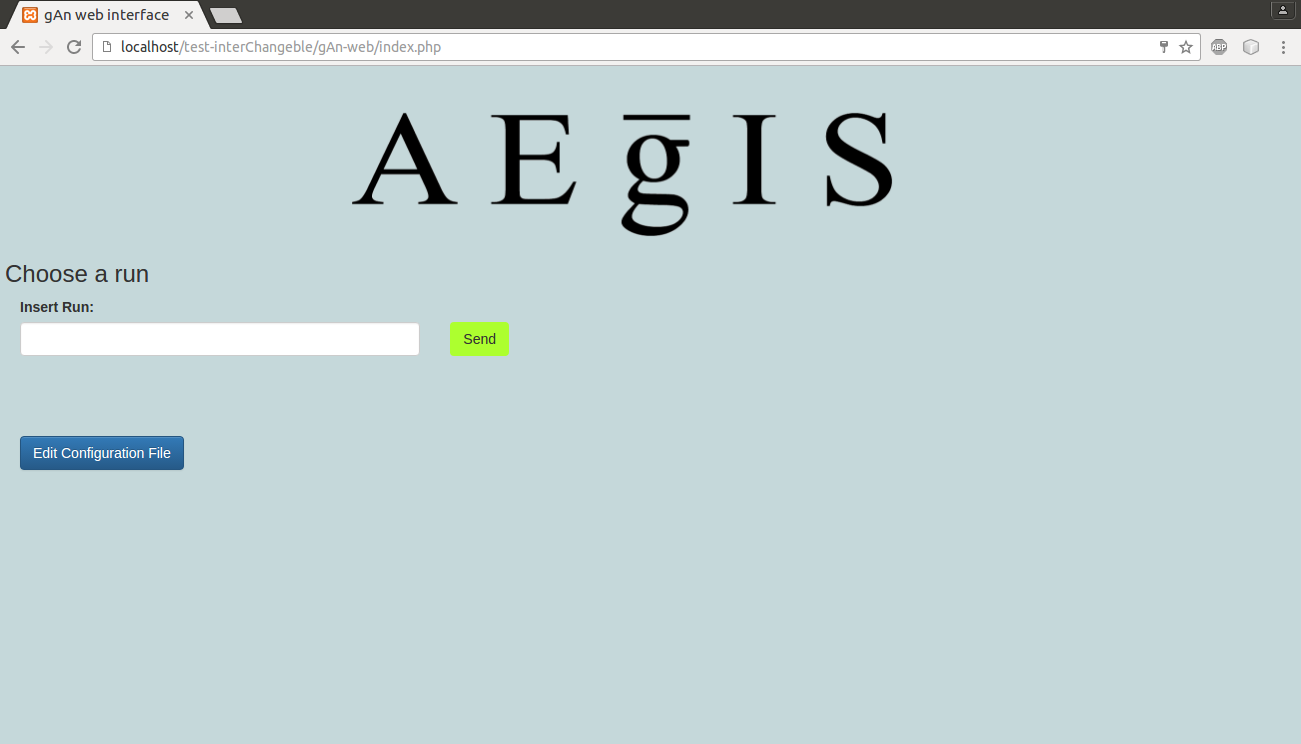
\includegraphics[scale=0.25]{HomePageOLD.png} 
\caption{The early homepage of gAn Web}
\end{figure}

It is quite clear: There is the AEgIS Logo, an input field where the user can insert a run number (only one in this version) and a "Send" button to start the analysis (using gAn). A button "Edit Configuration File" allows the user to  enter in the page dedicated to the configuration of the program.

\item The text output page:

\begin{figure}[H]
\centering
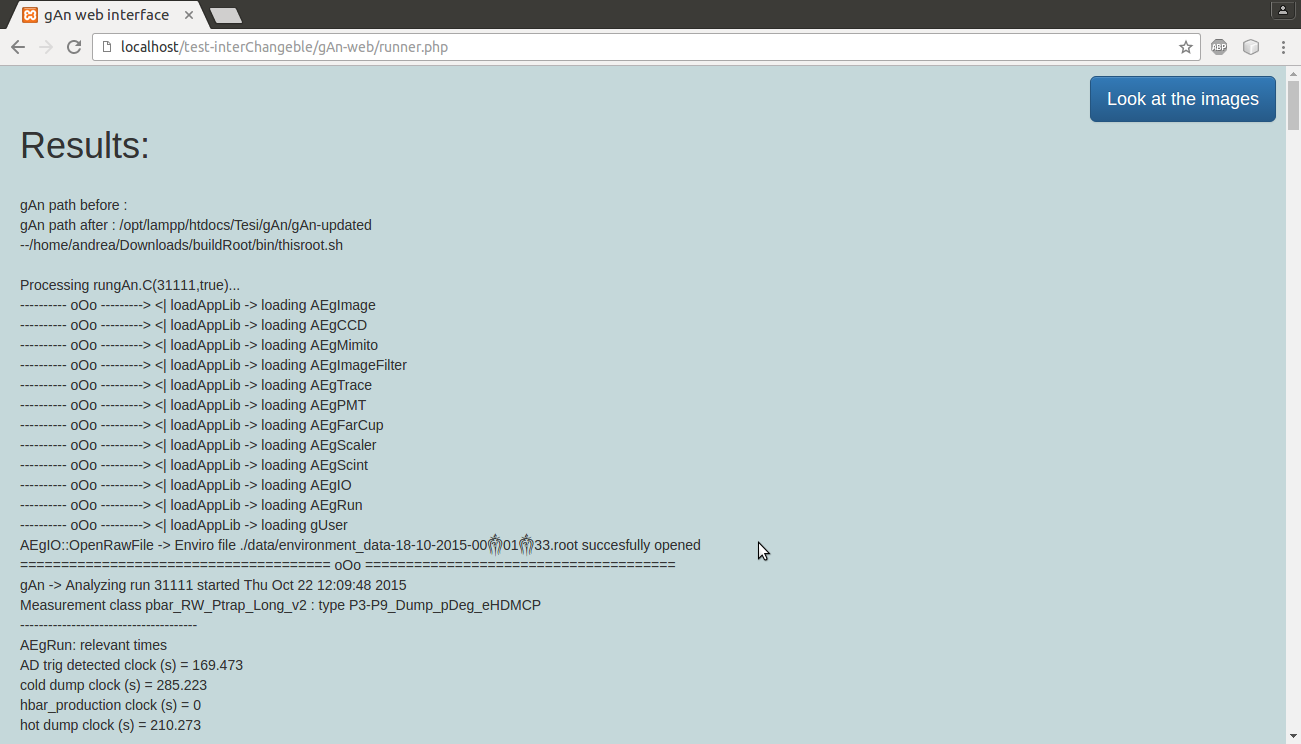
\includegraphics[scale=0.25]{TextOutputOLD.png} 
\caption{The early page related to the textual output of gAn Web}
\end{figure}
  
The textual result of the computation is visible: it seems to be too long and incomprehensible, but for physicists it is quite clear. The graphics is very minimalist, there is only one button: "Look at the images", that sends the user to the page related to the images. 



\item The page related to the images:

\begin{figure}[H]
\centering
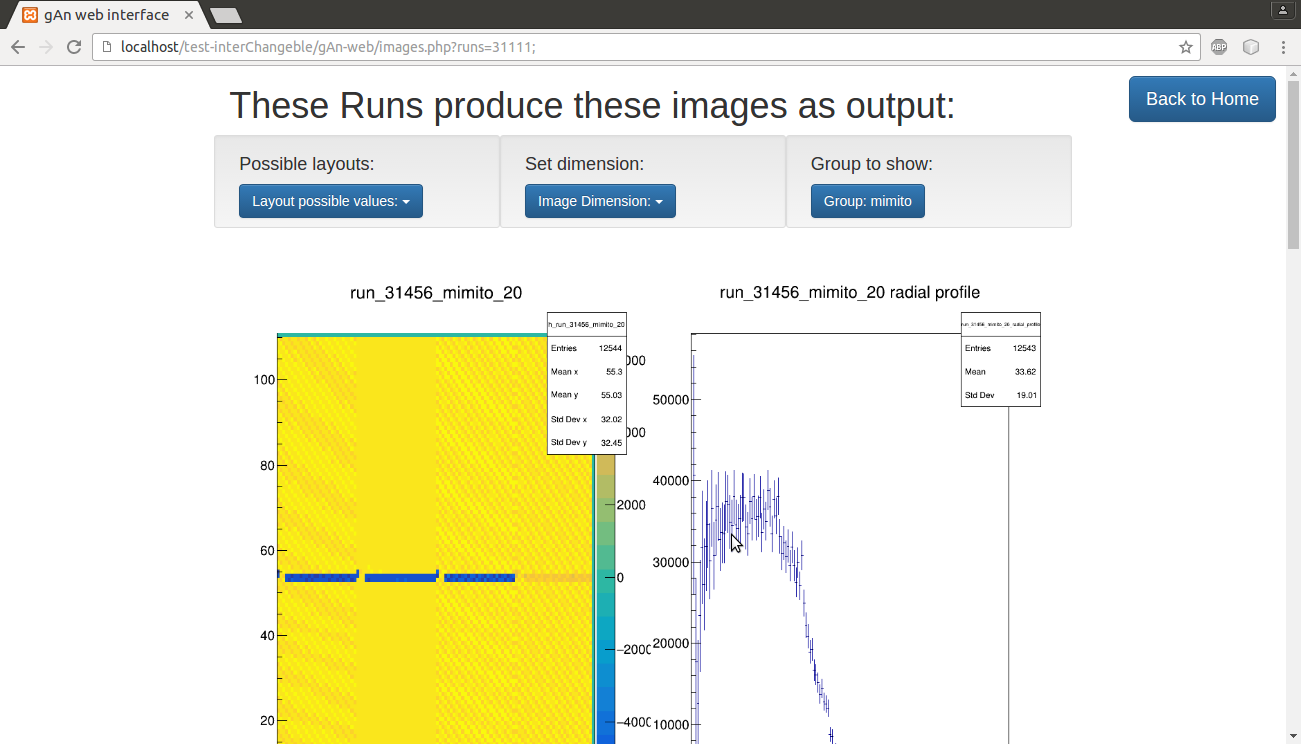
\includegraphics[scale=0.25]{AllImagesPageOLD.png} %TODO %TODO %TODO %TODO %TODO %TODO %TODO %TODO %TODO %TODO %TODO %TODO %TODO %TODO %TODO %TODO %TODO %TODO %TODO %TODO %TODO %TODO %TODO %TODO %TODO %TODO %TODO %TODO %TODO %TODO %TODO %TODO %TODO %TODO %TODO %TODO %TODO %TODO %TODO %TODO %TODO %TODO %TODO %TODO %TODO %TODO %TODO %TODO %TODO %TODO %TODO %TODO %TODO %TODO SISTEMA STOCAZZO DI IMMAGINE
\caption{The page able to show the output images in the early prototype}
\end{figure}   

This page shows the images in a dynamic framework, that the user can edit.
The user can choose by dropdown menus the dimension, the layout ("vertical", if he prefers the images disposed vertically one above the other, "carousel" if he prefers the images organized horizontally, navigable by a "next" button and a "previous" button), the group to show (each image belongs to a group, each group usually is composed by 2-3 images). Clicking on a image the user can open it in a full page version (but it is still a static image, a png).



\item The page that aims to edit the configuration file:

\begin{figure}[H]
\centering
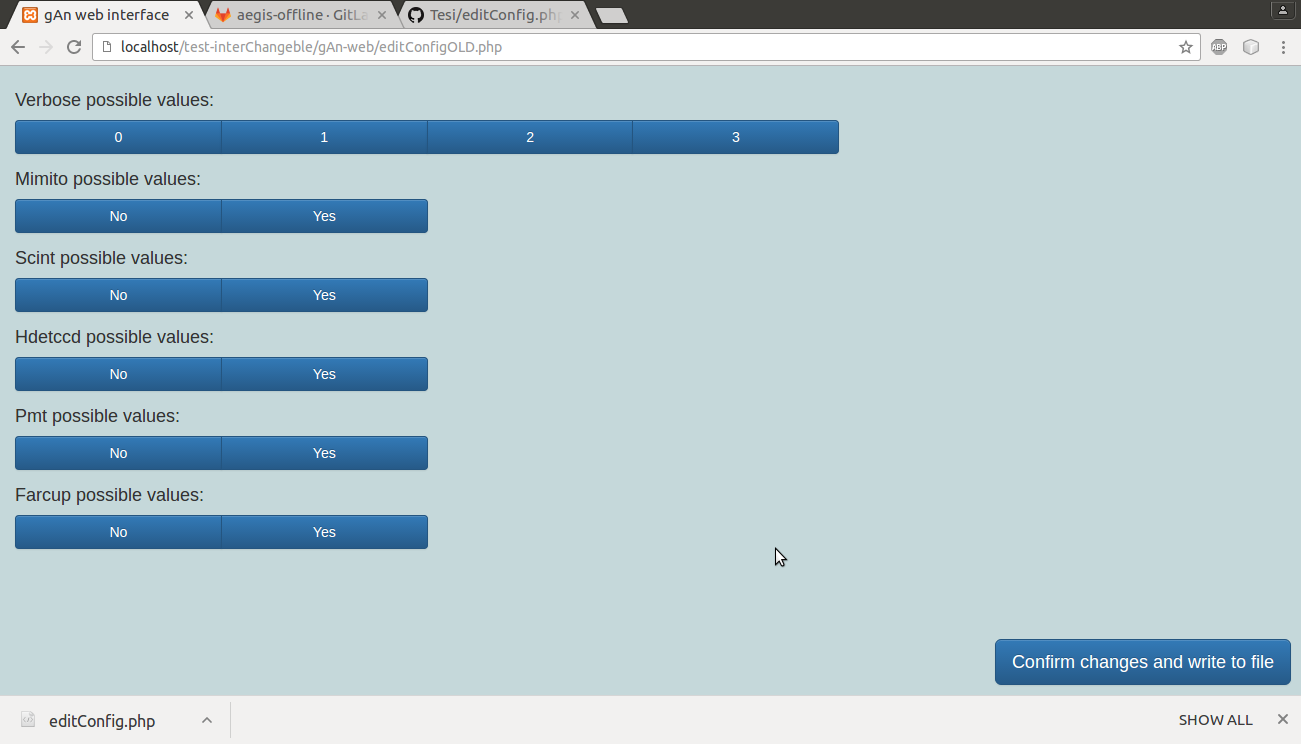
\includegraphics[scale=0.25]{EditConfigOLD.png}  
\caption{The configuration page}
\end{figure}   

This page allows the user to choose by radio buttons (modified using Bootstrap graphic) the value to insert in the configuration file of gAn. Radio buttons force users to insert correct values.    

\end{enumerate}

\section{How the early version can be improved}
The early version's goal is just to be a demo. In particular, it is based on the assumption that the user knows in every moment all about gAn (how does it works,  what is the meaning of each field of the configuration file, etcetera). It can be improved literally in every point, according with the principles of the Human Machine Interaction.


\section{Late version}

The late version is based on the early version, some pages (and functionalities) are added, some existing pages are improved. Following all modifications are explained.

\subsection{Modified pages}
The homepage:

\begin{figure}[H]
\centering
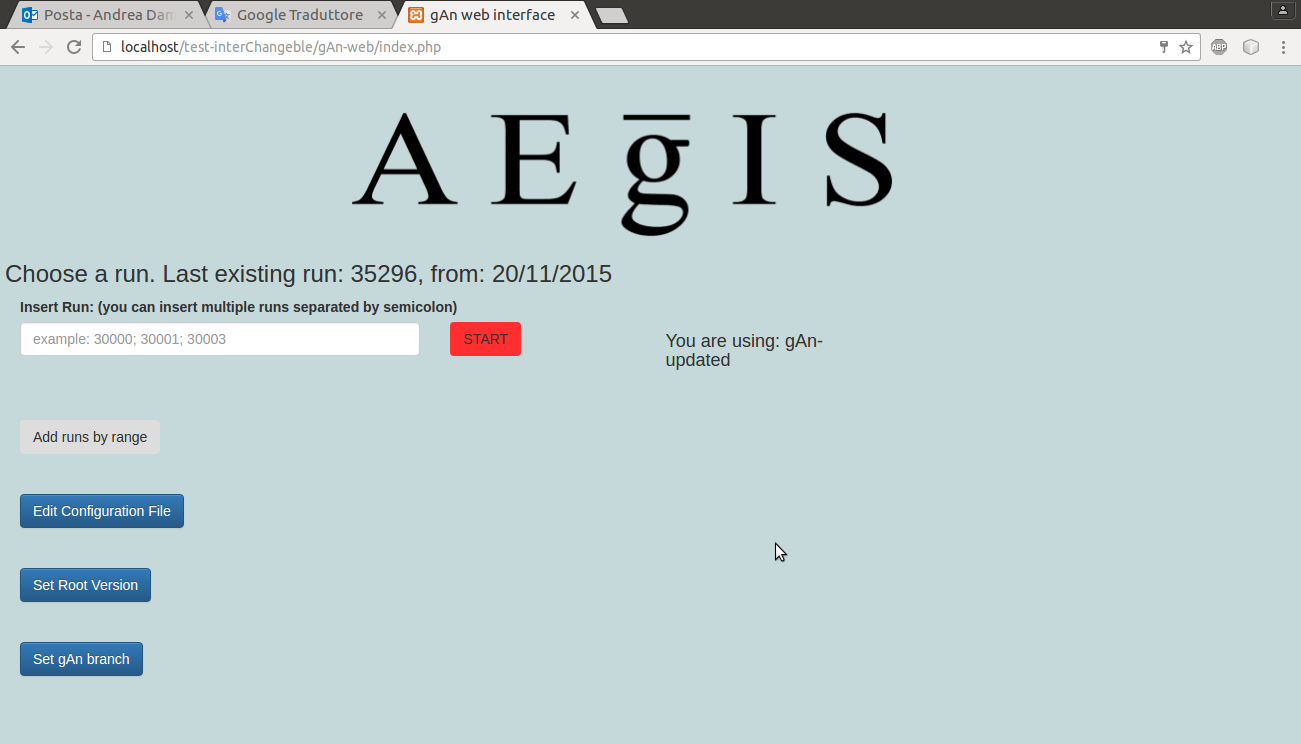
\includegraphics[scale=0.25]{HomePageEmpty.png} 
\caption{The homepage of gAn Web without input}
\end{figure}


\begin{figure}[H]
\centering
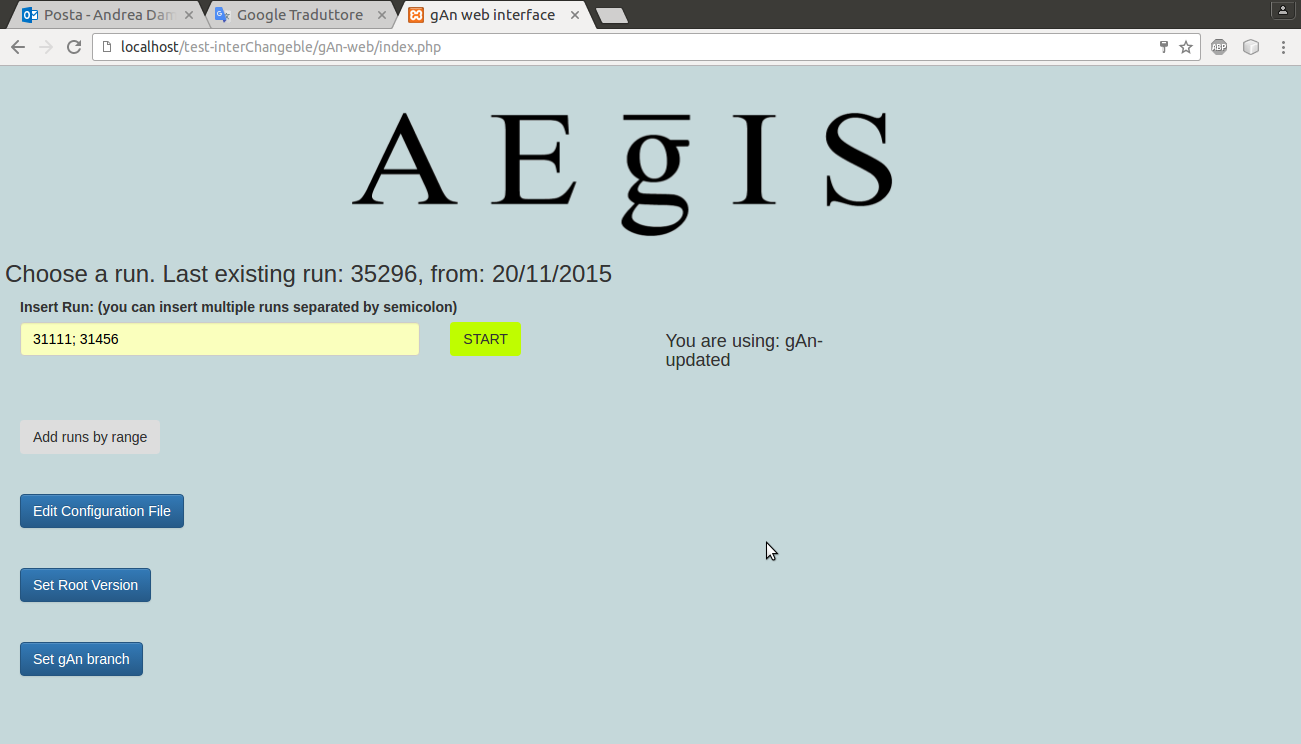
\includegraphics[scale=0.25]{HomePage.png} 
\caption{The homepage of gAn Web ready to start}
\end{figure}

There are some modifications:

\begin{enumerate}

\item The user is informed about what is the last existing run: he can read "last existing run: nnnnn, from dd/mm/yy". This point is important because in most cases the user searches results regarding the lasts 10 runs.

\item The button named "send" was unclear, the word "START" is more clear, the user can immediately understand that the goal of this button is to start gAn. The button is red and unclickable if there are problems (like in the following image) with the inserted runs (or if the input field is empty), green and clickable if there are no problems.	

\begin{figure}[H]
\centering
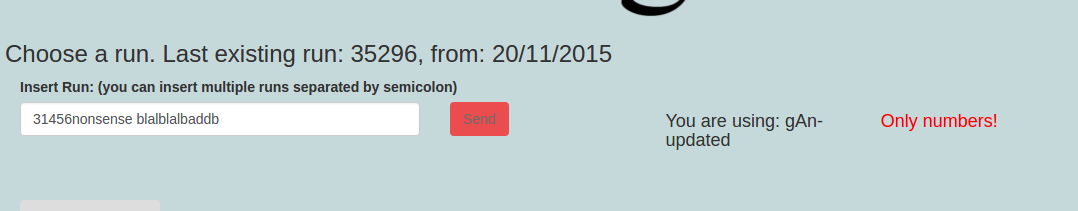
\includegraphics[scale=0.25]{ErrorInputHomepage.png}  
\caption{The "Start" button is red if the values in the input field are invalid}
\end{figure}

When the user clicks start a progress bar appears. Unfortunately it is very hard to understand exactly how long the computation will last, because different runs can take different time (it depends on the amount of data that the sensors take about the run, and on the workload of the server machine, that is in common with other applications). On average is observed that the computation take five seconds multiplied by the number of selected runs, but if another user asked for that computation before the system already has the results in memory and the computation is faster. A wait of several seconds can be not comfortable for the user, the progress bar is imprecise but ensure to the user that the system is working correctly to ensure the correct answer. In the following image the progress bar:

\begin{figure}[H]
\centering
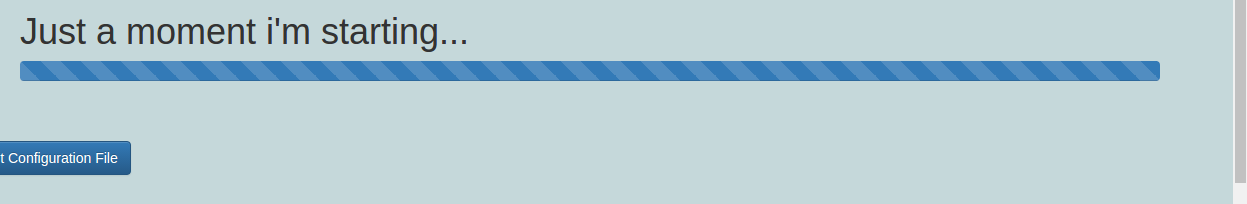
\includegraphics[scale=0.25]{ProgressBar.png}  
\caption{The progress aimed to make more comfortable the user's waiting}
\end{figure}



\item The input field has a place-holder, that shows to the user how to correctly insert the runs separated by semicolon (there is an automatic system that corrects the inserted values if the separator is not a semicolon)
 
\item It is possible to insert a group of runs selecting them by range (inserting the first and the last): the button "Add runs by range" opens a modal (shown in the image). The user can choose the minimum and the maximum of the range, the system validates the inserted values (maximum must be more that minimum, they must be numbers etcetera).

\begin{figure}[H]
\centering
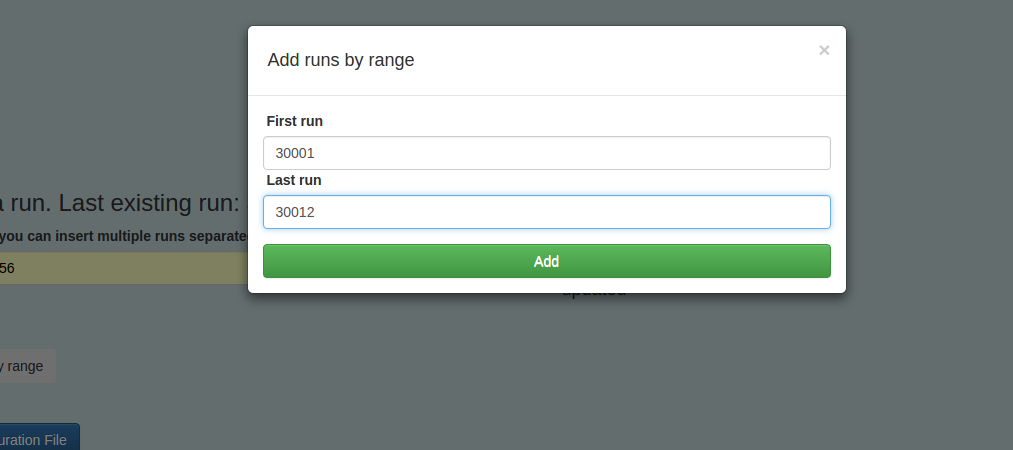
\includegraphics[scale=0.25]{RangeRunsModal.png}  
\caption{The modal opened by clicking the button "Add runs by range"}
\end{figure}

\item There is a little message "You are using: nameOfGAnBranch" that informs the user about which is the branch of gAn used by default if he doesn't change the configuration (the default branch is the last used, because usually when a group of users starts to use a branch, it continues to use it for some days)

\item There are two new buttons: "Choose Root version", "Choose gAn version". These buttons redirect the user to pages able to modify the version of Root and gAn used in the computation.
 
\item Each button and each field have a tooltip: a little explaining text that appears when the user moves the mouse over the object. In this way an inexperienced user can easily understand what each component does.  

\end{enumerate}


The page related to the modifications of the configuration file of gAn:

\begin{figure}[H]
\centering
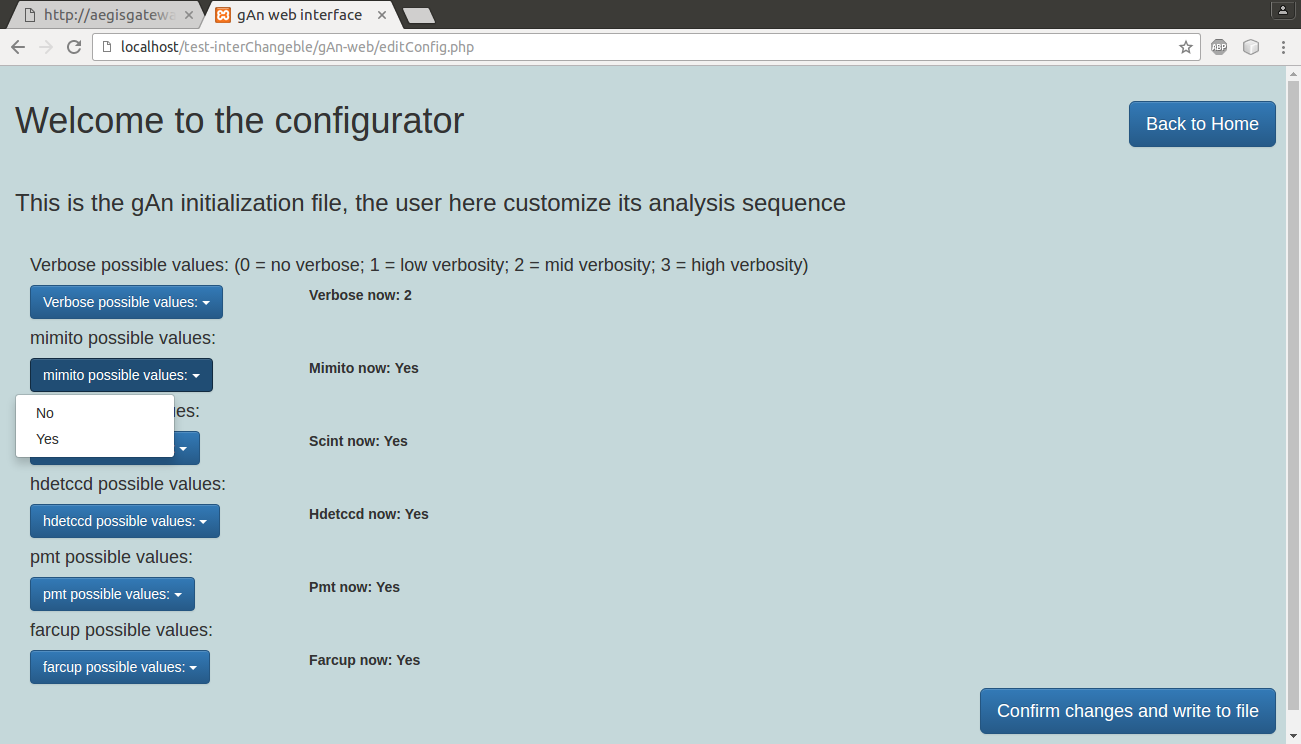
\includegraphics[scale=0.25]{EditConfig.png} 
\caption{The edit-configurator page of gAn Web}
\end{figure}

This page doesn't use anymore radio buttons, because some users ask the developers to use dropdown menus (for aesthetic reasons). The user can read near the button the currently selected value for each field. There aren't tool-tips able to describe the signification of each field here, because the users to which gAn Web is intended have a perfect understanding of the names and the features of each sensor (mimito, scint, farcup, etcetera are sensors).  



The page that shows the textual output of gAn is exposed in the following images, has some modifications:

\begin{figure}[H]
\centering
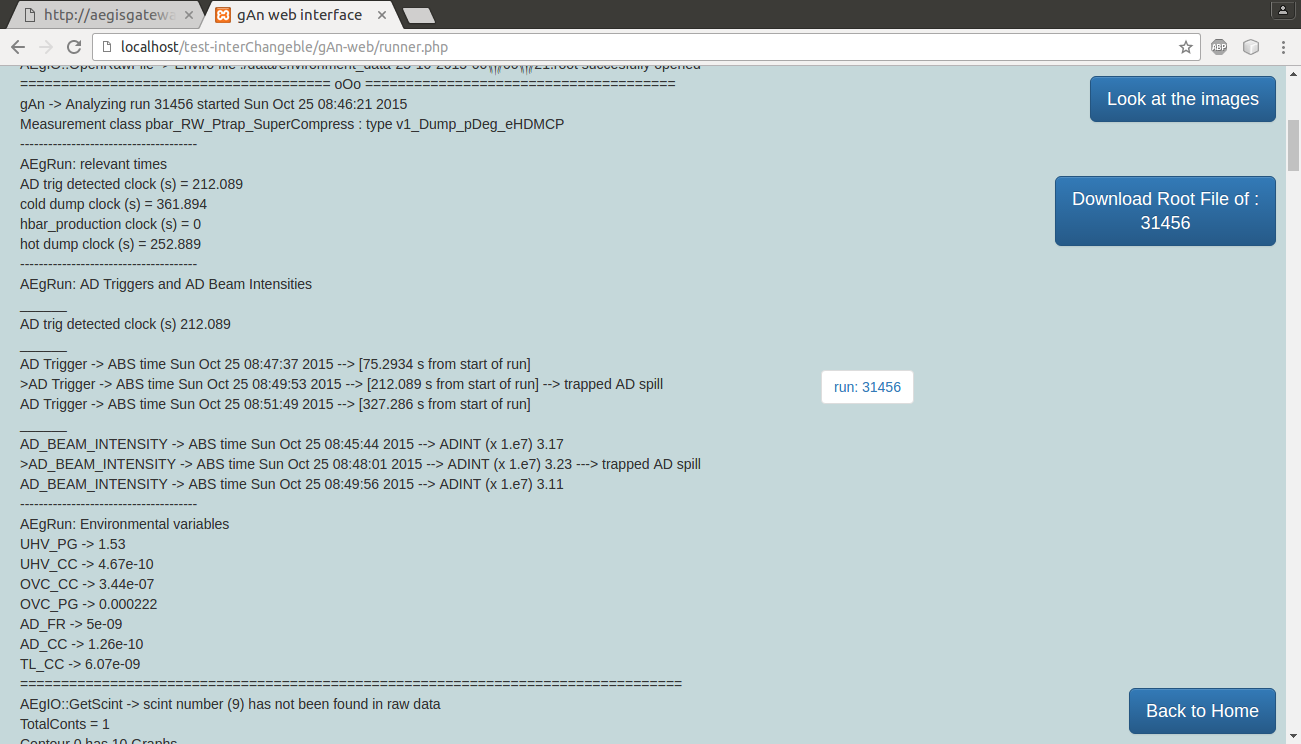
\includegraphics[scale=0.25]{TextOutputPage.png} 
\caption{The page who shows the textual output of gAn}
\end{figure}


\begin{enumerate}
\item The user can choose what results he wants to show on the screen by clicking the corresponding run number from the "navbar", like in the image:

\begin{figure}[H]
\centering
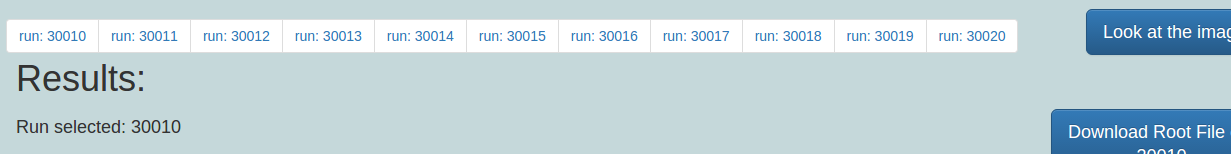
\includegraphics[scale=0.25]{WhichRunNavbar.png} 
\caption{By this "navbar" the user can choose the run results to show}
\end{figure}

This navbar is in fixed position related to the screen, and can be dragged by the user to allow him to decide where put it.

\item "Download Root File of: nnnn" is a button that allows to user to download the semi-processed file .root with some output information regarding the computation.

\item "Back to Home" gives the user the opportunity to directly return to the homepage. 

\item "Back to Home" and "Look at the images" are in a fixed position on the screen: also if the user scrolls down or up the screen he is always able to see these buttons.    

\end{enumerate}
The page that shows in an organized way the images that gAn produces in output. The following image shows the new appearance of the page:



\begin{figure}[H]
\centering
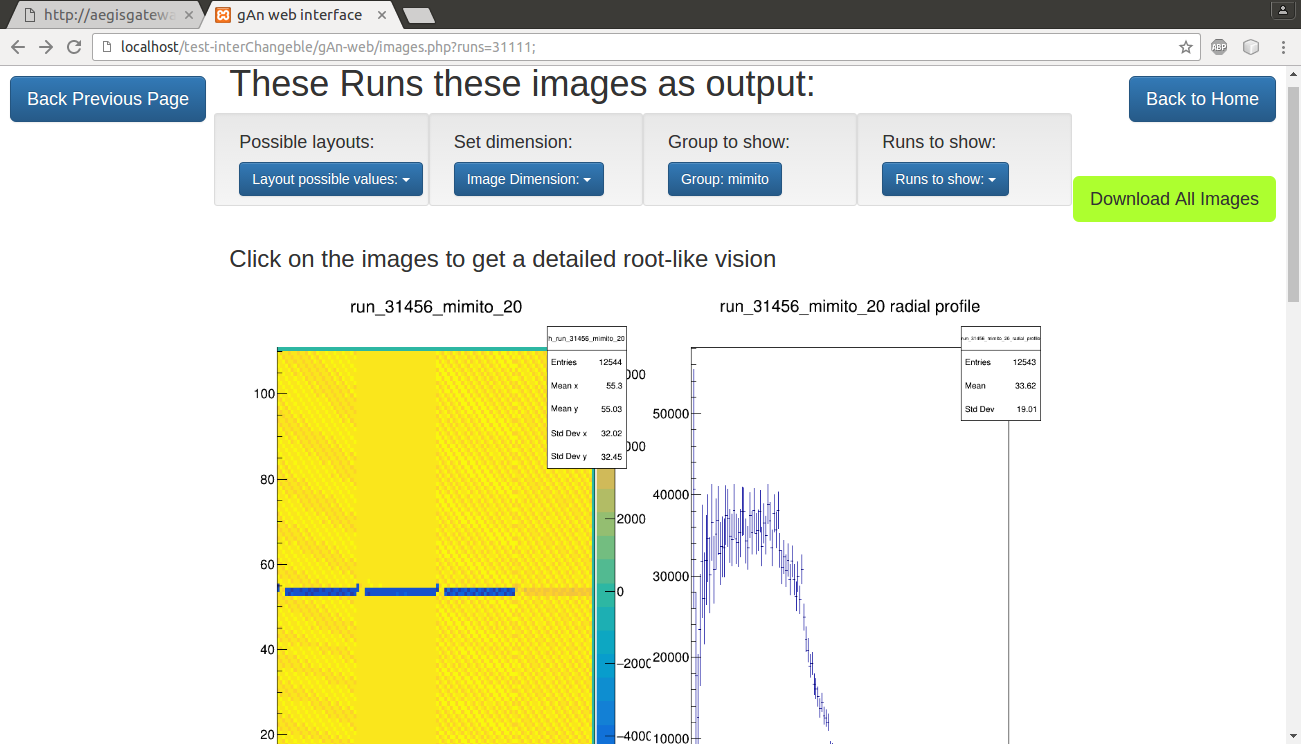
\includegraphics[scale=0.25]{AllImagesPage.png} 
\caption{This page shows all the images that gAn produces in output}
\end{figure}


Modifications:
\begin{enumerate}

\item The dropdown menu "Runs to show" allows the user to select only the images produced by a single run (by default the system shows the images related to all the runs). The users widely use this option, because in this way they can compare images extrapolated in the same way but related with runs with different configurations.

\item "Download All Images" allows the user to download by a single click all the images related to the execution. The late design introduces this requirement because commonly the users want to download the images using the right click of the mouse and the browser's button "Save Image As". In this way this process is faster and easier.

\item The buttons "Back to Previous page" and "Back to Home" are links towards the textual output page and the homepage. They are in fixed position.

\item By clicking on the image the user reaches a page that shows the image in full screen, but not in a static format: the image is dynamically accessible like shown in the following images:

\begin{figure}[H]
\centering
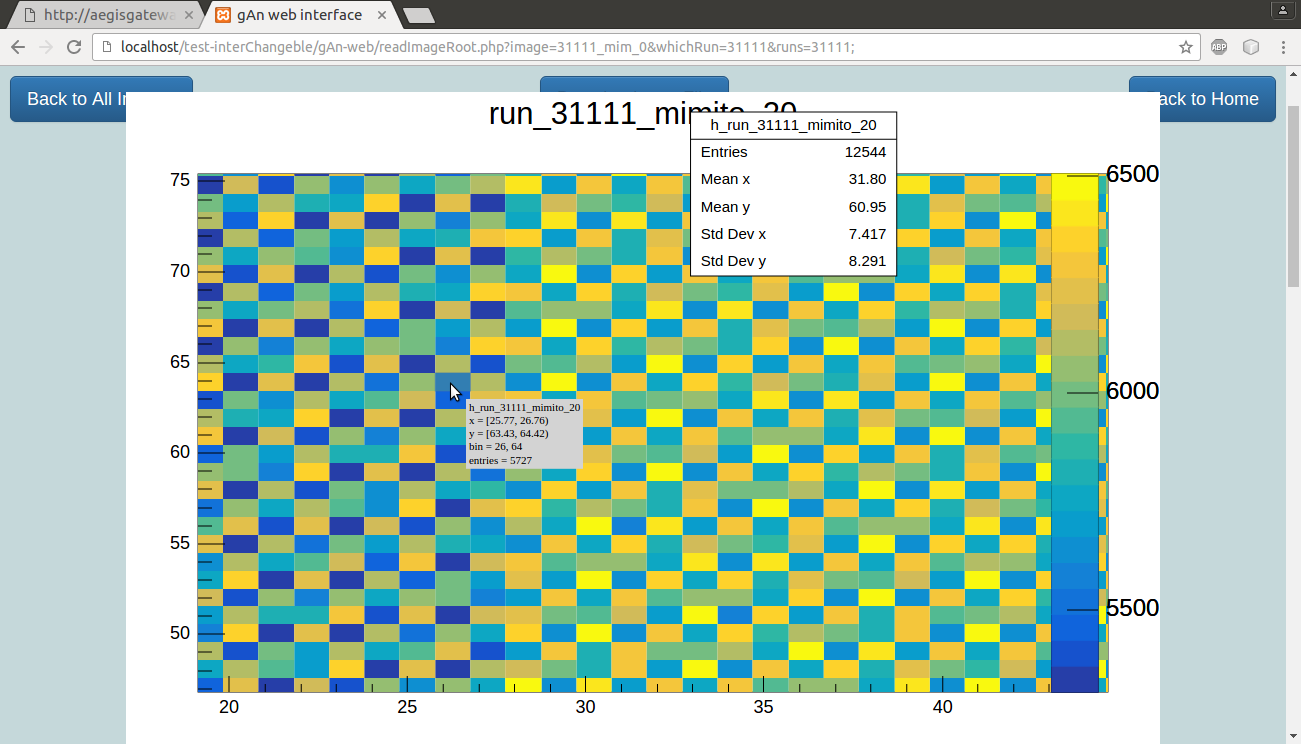
\includegraphics[scale=0.25]{RootLikeImage2.png} 
\caption{Moving the cursor the system shows the value of this histogram in the selected point}
\end{figure}



\begin{figure}[H]
\centering
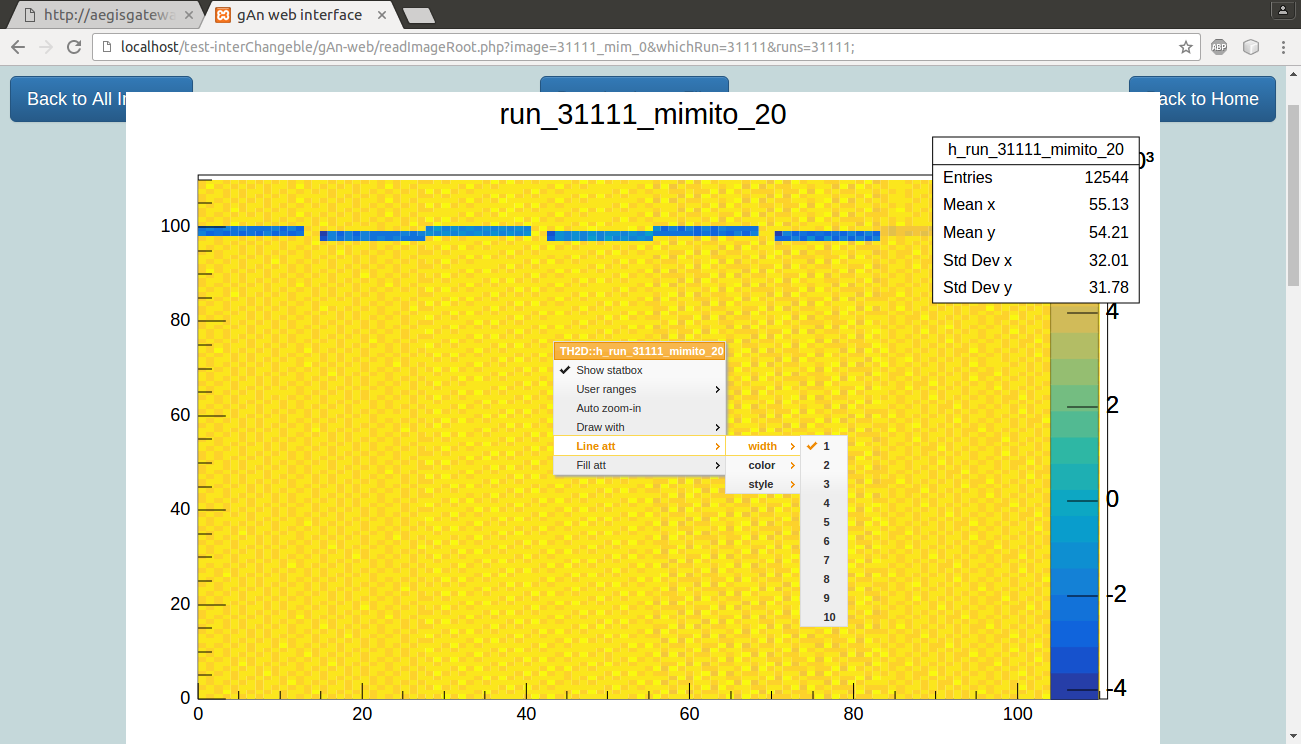
\includegraphics[scale=0.25]{RootLikeImage.png} 
\caption{The user can modify numerous settings in the generated image}
\end{figure}

\begin{figure}[H]
\centering
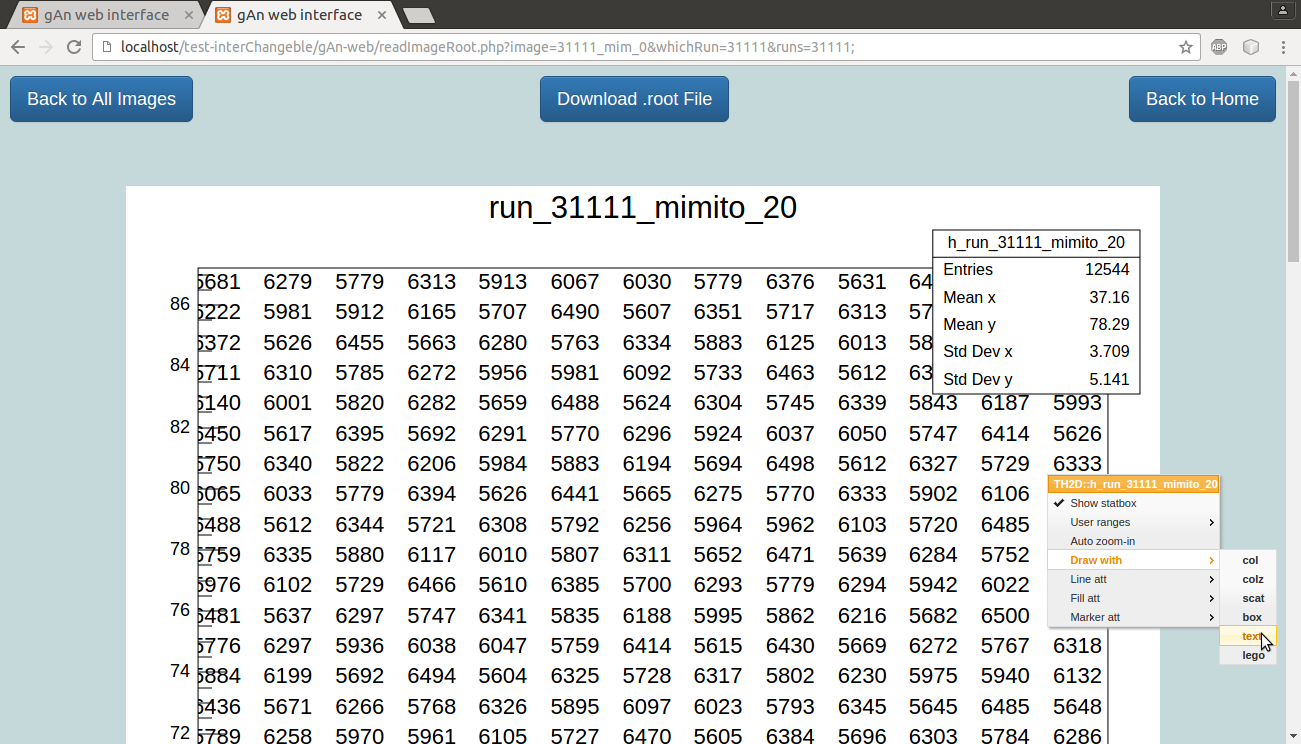
\includegraphics[scale=0.25]{RootLikeImage3.png} 
\caption{The user can show the histogram not only in traditional format, but also in a numerical format where the numbers are the value of the function in their position}
\end{figure}

\begin{figure}[H]
\centering
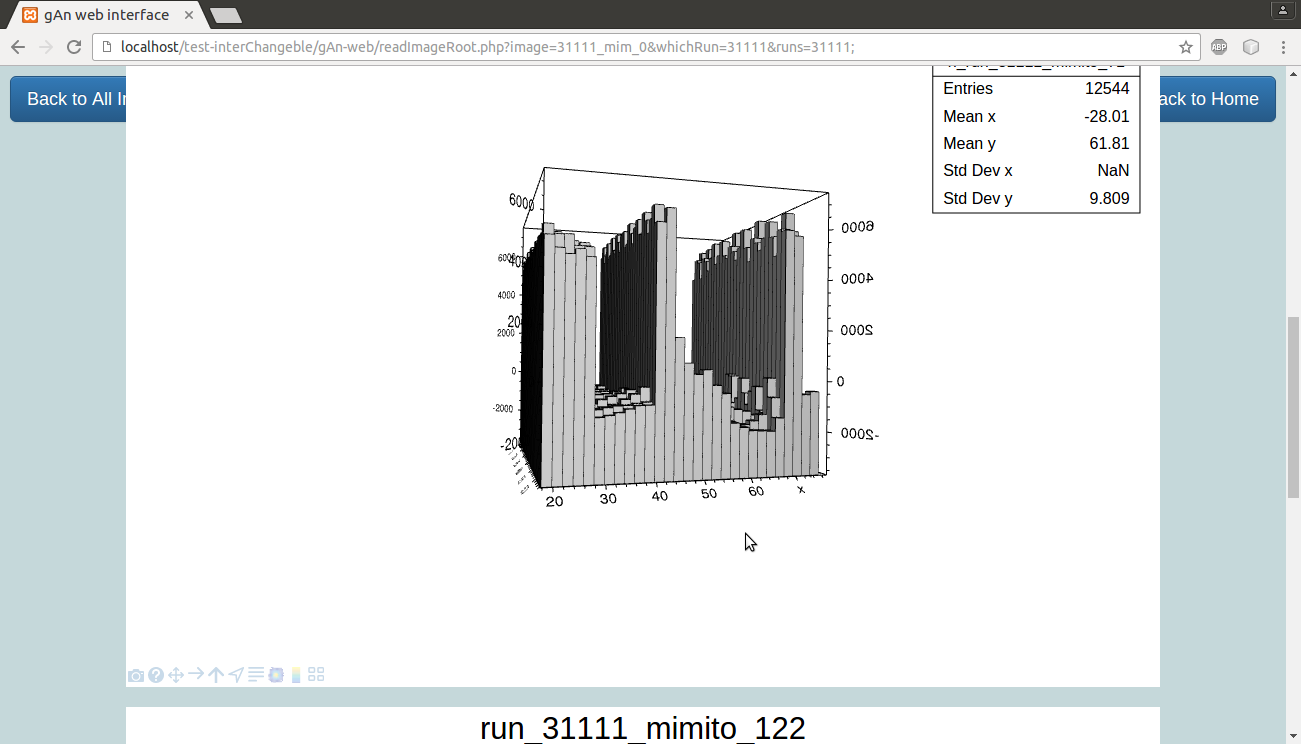
\includegraphics[scale=0.25]{RootLikeImage4.png} 
\caption{Another solution is to generate a 3d image in lego-style of the histogram}
\end{figure}


 
\end{enumerate}


\subsection{Added pages}

Some pages in the late version are completely new, because they implement new functionalities.

The first new page that the user sees is the login page. It is very simple, it doesn't authenticate a single user, but asks only the password of the office. This basic system of authentication aims simply to ensure that only the people that works in AEgIS experiment can use this software.

Following the login page image:

\begin{figure}[H]
\centering
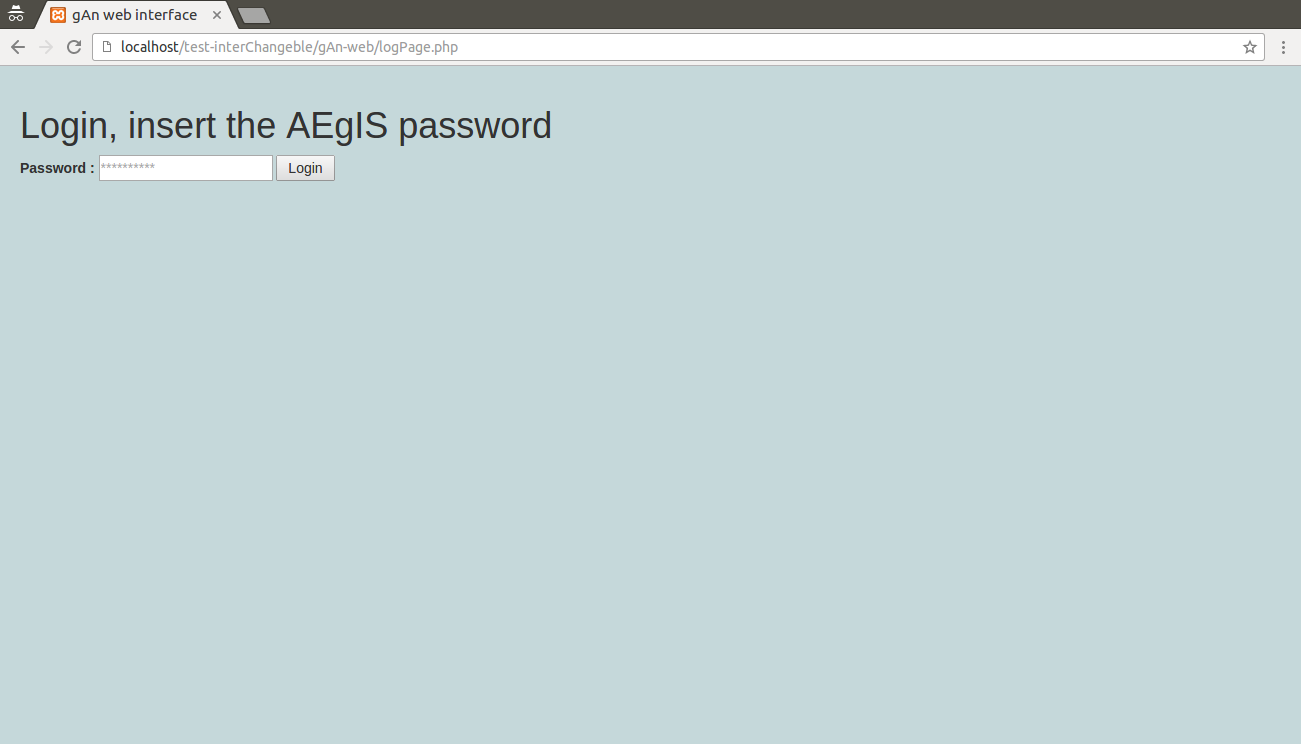
\includegraphics[scale=0.25]{Login.png} 
\caption{Simple login page}
\end{figure}

In the late version there is also the opportunity for the user to choose which branch of gAn and which version of Root Framework to use to execute the program. The pages that the user can user are quite similar, and quite simple. The user must use dropdown menus to make these choices, and there is always a default safe choice (the system remembers the last working version of Root and the last working branch of gAn), so it is impossible make errors or inconsistent choices. 

Following there are some screen-shots of these pages

\begin{figure}[H]
\centering
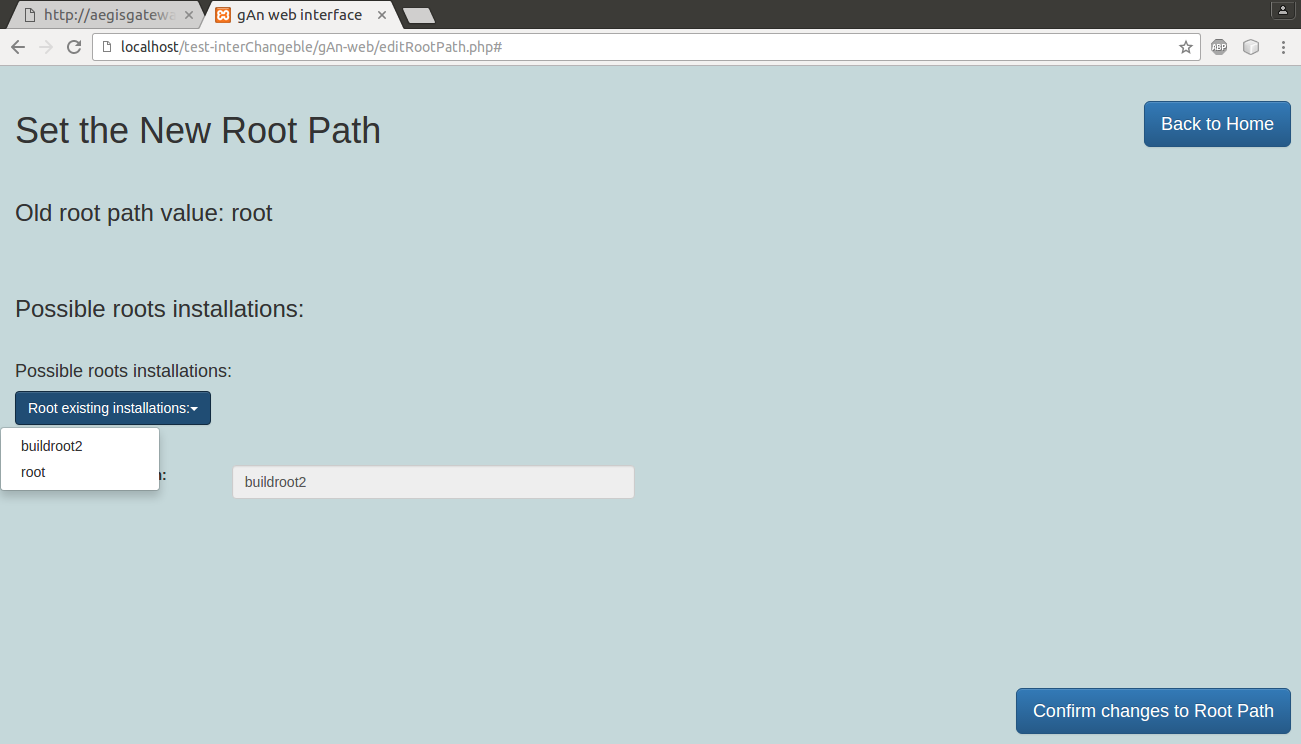
\includegraphics[scale=0.25]{RootVersionChoice.png} 
\caption{Page where the user can choose the Root version to use}
\end{figure}
 
 
\begin{figure}[H]
\centering
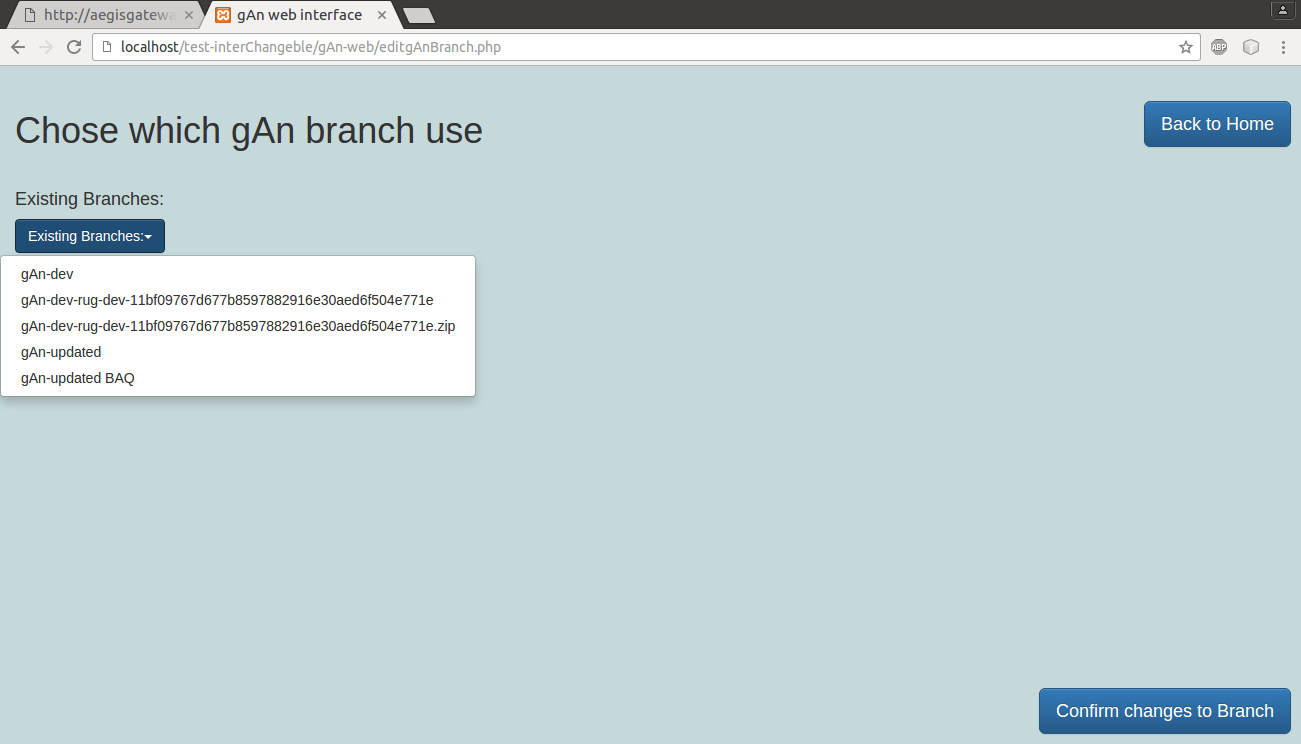
\includegraphics[scale=0.25]{ChoosegAnBranch.png} 
\caption{Page where the user can choose the Root version to use}
\end{figure}
% Chapter 1

\chapter{Final version} % Main chapter title

\label{Chapter5} % For referencing the chapter elsewhere, use \ref{Chapter1} 

Here will be explained the features of the final version, and how we are arrived at it.

\section{Functional requirements}

The last version (from now "gAn Web v3") is a modified version of the intermediate version. 
The second version's modification come from two sources: some adding requirements are proposed from the pilot users (that are also supervisors); These adding requirements are the following:

\begin{enumerate}
%1 chose analysis new way
\item 
The main kinds of analysis are now more clear: they are 4-5, and they are     quite stable. Their role and when they are useful is now steadily fixed. Each user, according on his task, knows (should know) in every moment which analysis fits better the situation, so, the best solution is allows the user to choose the type of the analysis through a dropdown menu directly in the main page (exactly like he chooses the run number). At this point the possibility of choose the gAn version is useless, because the definitive version of gAn include all the existing types of analysis. 

%2 single vs multiple
\item 
The kind of use of this software is quite different if you decide to work with a single run or a group of runs, so is better if at the beginning the user chose directly if he wants work with a single run or more than one. 

%3 don't choose root version
\item
There is an effort in the developing of the whole project to make it independent of the Root version, So the interface won't ask to the user to choose a Root version anymore.

\end{enumerate}
 
Furthermore, the version version with this last requirements was tested with the users: the developer studied their behavior observing them at work with the existing version, listening to their comments, and asking them opinion and information. The impact  of the debut with the users highlights some problems to be overcome, and from the analysis and the solution of these problems the requirement of the last version was defined. The problems observed (and for each the proposed solution) are the following:

\begin{enumerate}
\item 
It is important to help the user in some way to choose the run number: the user needs a view on the logbook of the run, that is a text in which there are information about each run number divided by date.

\item
Actually nobody use the button to modify the dimension of the images: they all use the biggest version.. is better to remove (or move in a less central place) this dropdown. A similar reasoning can be done for the dropdown that allows the user to switch between the vertical and carousel menu (everybody use).

\item
The read of the textual output takes too much time: it can be improved highlighting the most important parts (or better, the most important parts for the selected type of analysis)

\item
The user need to choose by the configuration page the degree of precision (the minimal error) of the x-axis (the time related axis) of each time-related values images. This parameter seemed to be not very important and in the second version actually there wasn't, but all the users modifies it quite often (manually). So is better to let them to do it by the interface

\end{enumerate}

\section{Non-functional requirements}

There is another special requirement emerged in this version, not strictly related to the common behavior of the interface but quite important: the machine  used as server is also used for the testing of single analysis when they are written; sometimes these analysis crashes (quite normal in a test phase), and they remain in a "hung up" state, without doing nothing but occupying Ram memory, and if the blocked application are numerous that can be a problem for the performances of the machine. To ensure a correct behavior gAn Web must check this situation at starting and eventually resolve it.

\section{Scenario based functional analysis}
TODO

\section{Prototypation}
TODO 

\end{document}  
